

\chapter{Literature Review}  

\noindent In this chapter we provide the technical background related for the context of the project.


\section{Large Language Models (LLM)}
Natural language processing (NLP) has always been an intricate field because of the complexity of how humans communicate. The meaning of a message
can vary because of homonyms, tone, context, and other factors that affect the message delivered. These are some challenges that computers face when trying
to replicate or learn human text communication and expressions.  However, this changed with the introduction of Large Language Models (LLM) \cite{naveed2024comprehensiveoverviewlargelanguage}.
These models are trained with large amounts of data to replicate human-like patterns or generate text based on statistical relationships between words, and these
advancements were made possible by transformers \cite{vaswani2023attentionneed}. Previous NLP techniques such as Recurrent Neural Network (RNN) and
Long-Short Term Memory (LSTM) could help in understanding a sentence's context in the short term. However, these struggle when trying to understand longer texts.
In contrast, transformer architecture, seen in Figure \ref{transformer}, differs from others because it uses self-attention.

\begin{figure}[!hb]
    \centering
        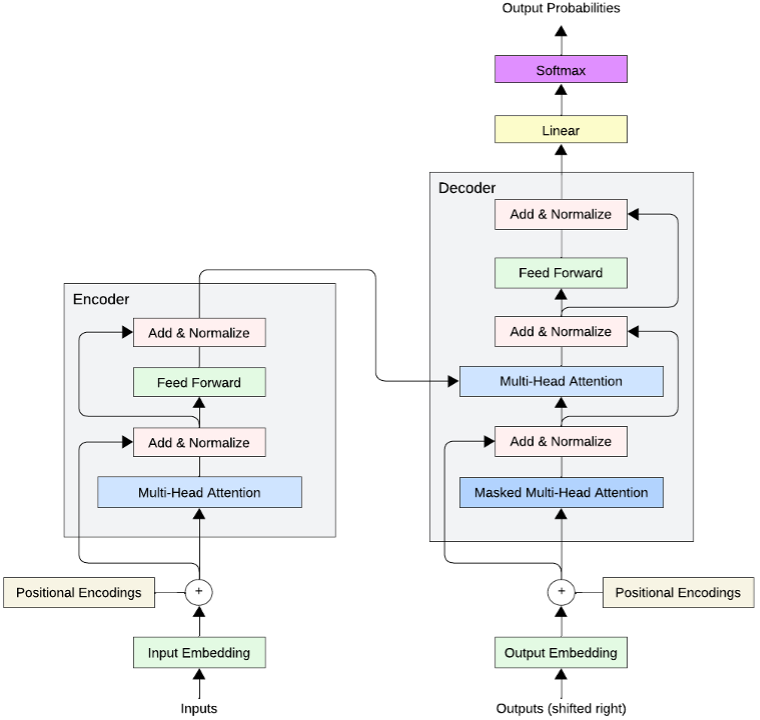
\includegraphics[width=1\linewidth]{images/transformers_architecture.png}
        \caption{The Transformer Architecture}
        \label{transformer}
\end{figure}

\subsection{LLM Architectures}
This self-attention finds dependencies between all words in a text, short and long-term. The process of this starts by turning words into tokens. A token can be a word,
subword, individual letter, or a sequence of words mapped to an embedding. The embedding is the vector representation of a token in high-dimension space; its size
depends on how much information it stores about the token. Now, self-attention finds relationships between all tokens and gives them an attention score, measuring
the relevance of a token to others. Transformers uses the scores to generate a final representation of each token. This process depends on how the models make a token.
The tokenization strategy is determined by the preprocessing stage, and influenced by the embedding and model architecture. The embedding impacts the strategy
because of its dimensionality, the amount of information encoded, and the model's sequence length limitations. In Figure \ref{transformer},  we can see an encoder and a
decoder in the transformer architecture. Based on that, there are different LLM architectures: decoder-only, encoder-only, and encoder-decoder. Each one has advantages
for specific tasks and limitations for others.

\begin{figure}[!hb]
    \centering
        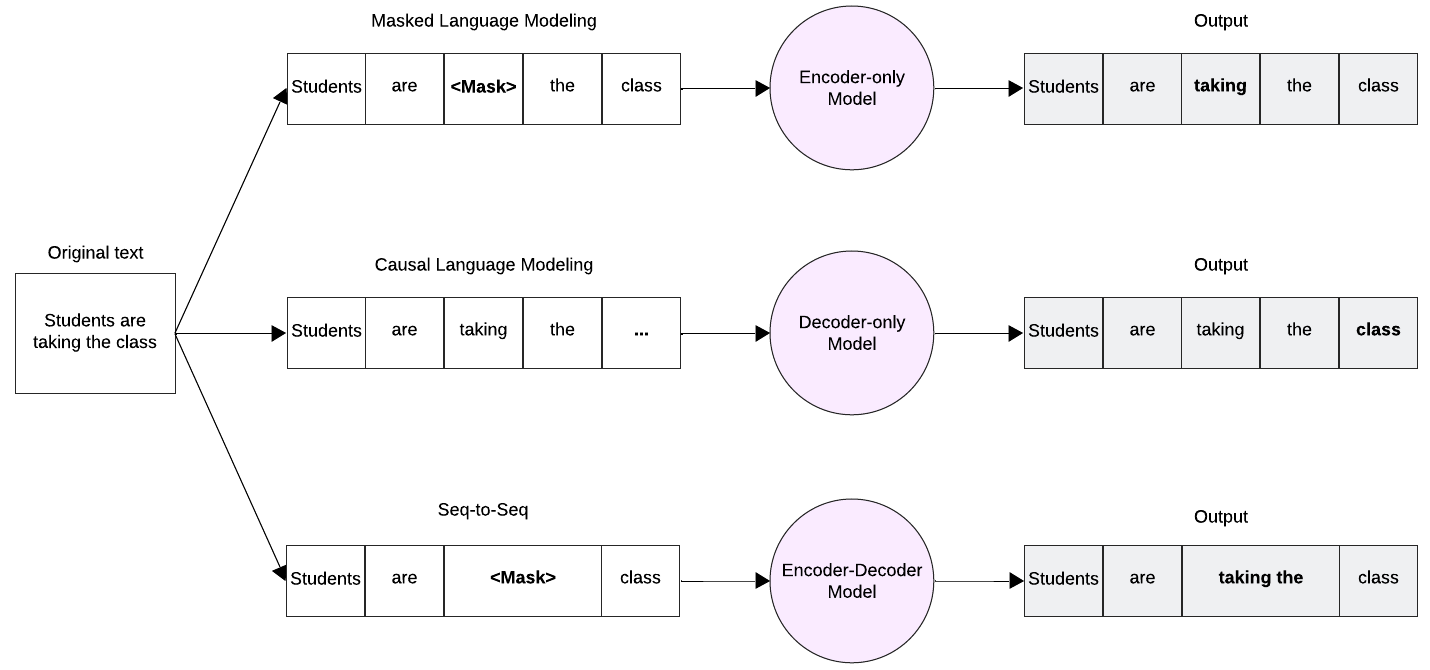
\includegraphics[width=1\linewidth]{images/LLM_Arch_text_generation.png}
        \caption{LLM Architecture and Comparison}
        \label{text_generation}
\end{figure}

\begin{description}

%\subsection{Decoder-only models}
\item[Decoder-only models:] Decoder-only models predict the next word based on the previous context, thus being unidirectional models. The model achieves this by taking a text or prompt as input and returning 
a first word. For each subsequent word, the model uses the previously generated text as input to predict the next word, continuing until it produces a coherent output. In Figure \ref{text_generation},
the model predicts the last word based on the previous context. Because of their ability to predict sequences of texts, they are frequently employed in tasks like summarization and text generation. Models
that perform those tasks are called causal language modeling (CLM) because they predict new tokens not found in the input. Compared to the other architectures, these models are massive
in size. Because of their sizes, these are not very practical or cost-effective for daily usage. These are the most commonly known models, such as GPT-3 \cite{DBLP:journals/corr/abs-2005-14165},
Mistral \cite{jiang2023mistral7b}, and LLaMa \cite{touvron2023llamaopenefficientfoundation}.

%\subsection{Encoder-only models}
\item[Encoder-only models:] These models predict by masking specific words in a sentence. Said masking helps them understand the meaning or relation of the masked word based on context. They are bi-directional,
which means they take the context before and after the masking to evaluate the word. The example in Figure \ref{text_generation} shows a sentence with a word mask being inputted to
the encoder LLM; the model predicts the missing word by using the surrounding text. That is why they tend to perform well at classification and sentiment analysis but are not optimal for text
generation. Said models are called masked language models (MLM). In contrast to other architectures, these models are relatively small. Some examples of encoder-only LLM are BERT
\cite{DBLP:journals/corr/abs-1810-04805} and RoBERTa \cite{liu2019robertarobustlyoptimizedbert}.

%\subsection{Encoder-Decoder models}
\item[Encoder-Decoder models:] These models combine masking and text generation. They work by masking the sequence of texts and using the context around it to make a prediction. As seen
in Figure \ref{text_generation}, they can mask more than one word from the original inputted text. Because the model generates sequences of texts, it is commonly used for translation
and question and answer. Translating between languages cannot be achieved through word-for-word conversion; it requires understanding the entire sequence to preserve the context.
To have an optimal model, both encoder and decoder must be trained for the task one wishes to achieve. Depending on the task, it can be harder to train compared to the other types of architectures.
Bart \cite{lewis2019bartdenoisingsequencetosequencepretraining} and T5 \cite{2020t5} are examples of encoder-decoder LLMs.

\end{description}

Knowing the architectures, each one has its advantages for specific NLP tasks. However, to perform these tasks, we must train them to do so.

\subsection{Classification tasks}
Large Language Models use different learning methods to train. Such methods include zero-shot, one-shot, and few-shot learning. As the name implies, zero-shot learning is training a model without
previous knowledge of the data; it is learning from scratch. One-shot learning is a method that receives one example as input and tries to generalize from that example. The final method uses
multiple examples to find a pattern between them. 

In Figure \ref{gpt_example}, we can see an example of zero-shot learning. This LLM has no previous knowledge of the task that it must perform. Nonetheless, the model used, GPT-3, has the 
advantage that it can follow instructions when redacted clearly. Here, we tell the model that it must act as a medical expert and identify if a message is health-related and why it is classified that way. 
Also, the result must follow a specific format. This process of instructions is called prompt engineering. Prompting does not retrain or adjust the model parameters. Thus, it does not always have optimal results.  
 
 \begin{figure}[!h]
    \centering
        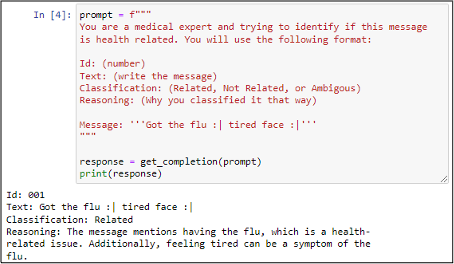
\includegraphics[width=0.9\linewidth]{images/gpt_example.png}
        \caption{Zero-shot example of GPT-3}
        \label{gpt_example}
\end{figure}


Moreover, LLMs that completed training with no additional modifications are known as based models. The response from this model will most likely make no sense with the premises it receives.
This happens because the model is trained on excessive texts to find patterns between them, but this pattern might not be on par with the input. For the model to return a coherent response, it must go through
a fine-tuning process. Fine-tuning consists of making a model perform specific tasks, such as chatting, summarization, chatbots, and others. To fine-tune a model, it must undergo another training process, with
training data related to the tasks it will perform. However, there are multiple training types. We will focus on Sequence Classification and Causal Language Modeling.

\begin{itemize}
\item{\textbf{Sequence Classification:}} This involves predicting a class label based on an input. That label is a number associated with a class. All previously mentioned models can be trained for Sequence
Classification, which is the most common training type.

\item{\textbf{Causal Language Modeling:}} This training is used for the model to learn the context of the text. We use this so the model learns to generate a text answer based on the input. The labels are texts related to the input.
This type of training is similar to question-and-answer problems, in which the model infers a result based on the question. CLM is more expensive in computing power than Sequence Classification because 
the labels must be embedded. That training type is most commonly used in models that have decoders because they are usually used to generate texts.

\end{itemize}

A problem with fine-tuning LLMs is that they require excessive computational resources to train or fine-tune. It is not viable to fine-tune all the parameters in the model to perform a specific task. However, there is an
alternative to fine-tuning a model without having a resource problem.


\subsection{Low-Rank Adaptation (LoRA)}
The research in \cite{hu2021loralowrankadaptationlarge} created a technique to train models with billions of parameters effectively. Their technique, LoRA, helps reduce the amount of computational resources and
parameters to train while maintaining optimal performance. LoRA trains specific layers of the model instead of retraining the full system. Their research shows that they reduced the GPT-3 training size from 350GB to
35MB. However, a limitation of LoRA is that we must add the trained layer to the base model. That means that after training, we use both the base model and this adapted layer to perform a task. Nonetheless, it is still an
improvement when they reduced the resources used by 3x, and their model had an accuracy of \textpm 0.5\% compared to full fine-tuning. An effective fine-tuning process is possible, but we need to see some use
cases for these models.

\subsection{Example Applications}
The authors in \cite{koh2023groundinglanguagemodelsimages} trained a based LLM model to understand images and give a text description or a combination of text and image. The training process for
the model used images and their captions as their data and the zero-shot learning strategy. Their resulting model was used as a chatbot that identifies images, answers questions, or gives
visual examples. Another experiment was \cite{inproceedings}, where the authors trained a model to identify sentiments on financial market decisions. In this case, they used prompting, also called in-context learning, for 
the model to answer the sentiment of the texts. In-context learning does not update any parameter of the original model. Their model resulted in a 70\% accuracy on sentiment prediction, failing mostly on neutral posts.
A possible problem with the neutral post is that prompting does not train the model to perform a specific task. That experiment showed the problem that users face when they use social media to make decisions.
They clarified the importance of not taking the model for granted and how social media can cause a user to make a poor decision.

\subsection{Challenges and Limitations}
An issue with LLM is that they answer based on statistical relationships between words, and occasionally, their output could make no sense. Sometimes, they can generate a result that is not factual
or valid; this phenomenon is called AI hallucinations. These models train to find patterns between tokens. Without the proper context, they cannot differentiate between fact and fallacy. This context
needs to  be related or similar to the input that the model receives. However, finding the necessary information is not optimal if done manually. That begs the question, how much data would be needed
to achieve a coherent answer, and how can this be done effectively?


\section{Vector Databases}
AI hallucinations occur when models generate a plausible output but lack factual accuracy. We can minimize the hallucinations by providing context relating to the text inputted. A solution to this
is finding data from officials or experts on the topic associated with the text. Given the vast amount of research available, narrowing down relevant information becomes a challenge. In addition,
the context quality is essential for the model to make any inference. The search process for this consumes time and is not always optimal. 

Nonetheless, if we have an immense amount of data from different sources, we can benefit by using a vector database. In contrast to other databases, they store data in a vector representation.
These databases can come in different forms, like Chroma \cite{chroma}, a native vector database. Also, some relational databases have extensions that allow them to make vector similarity searches,
like Postgres with pgvector \cite{pgvector}. They can turn images, videos, documents, and others into numerical embedding. These embeddings are numerical vectors capturing semantic meaning \cite{10455990}.
They are practical because the system stores the data provided as vectors in a high-dimensional space, where semantically similar data are positioned close in said space. We can see a text example of the vector
space in \ref{vector_space}. If we search for "Flu" it could return "Sick" or "Covid" with a higher probability than "Car" or "Truck". As we can see, querying this database will return a result close to the input.

  \begin{figure}[!h]
    \centering
        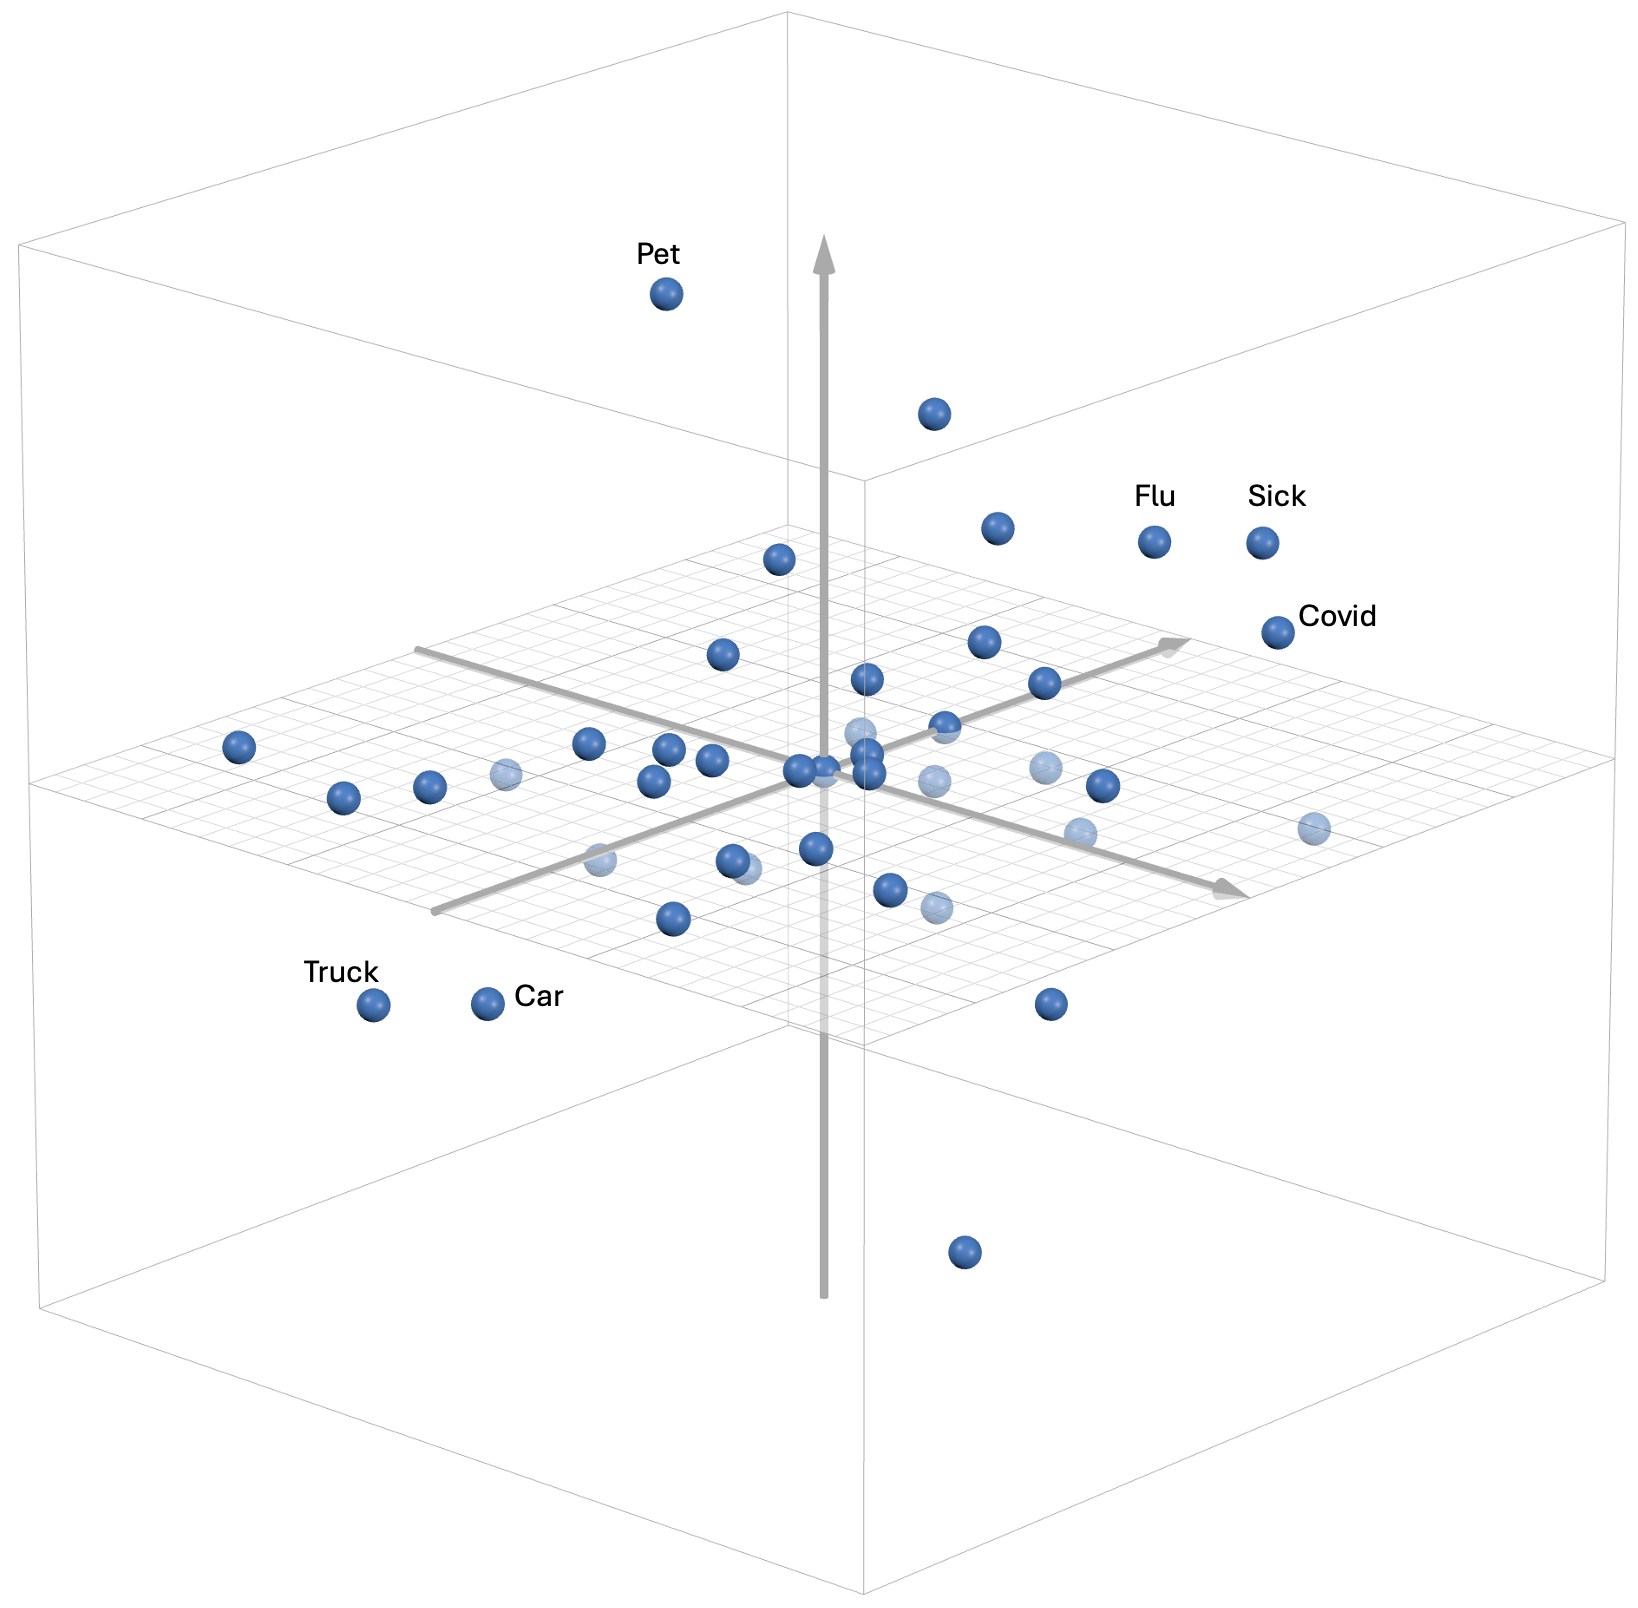
\includegraphics[width=0.85\linewidth]{images/Vector_example_update.png}
        \caption{High-Dimensional Space Representation}
        \label{vector_space}
\end{figure}

Although these systems help find similar text, there are a few limitations. One such problem is the vector size, which can impact the accuracy and resource usage \cite{han2023comprehensivesurveyvectordatabase}. If
the vector size is relatively big, the system will have a higher accuracy but will require more storage and resources to process. Also, this affects when searching large datasets, which incurs a resource-intensive search.
 
For the data insertion process, we need to find optimal strategies for our data. If we focus on a text dataset, the best practice is to split the document into chunks. This splitting process must be optimal for the task we want
to achieve. If we split it into small chunks, it will have a more precise answer, but we dilute the meaning of the text. On the other hand, larger chunks can have more context but less relevance. After selecting the appropriate
size, these chunks must be turned into a vector, usually done with an LLM. Finally, we store these vectors and their chunks in the database system. 

To search the system, we send a query to the LLM that converts it into a vector. Then, the vector is used in the database to make a similarity search. The system will return chunks that can function as context for an LLM to
analyze. In this context, an LLM can use the retrieved chunks to generate a fact-based answer from outside their initial training. This process, known as Retrieval-Augmented Generation (RAG), enables LLMs to access relevant
information during text generation. In \cite{10683437} they tested LLM to answer a test that contained images and text. They evaluate the GPT3 base model, the base model with prompt, and a GPT3 with RAG. Their experiments
showed that the base model's average success ratio was 40\%, the second model was 58\%, and the model with RAG ended with 75\%. Said experiment showed that an LLM can outperform when it receives the necessary context.
Therefore, RAG can assist in providing expert-level responses, but human oversight is still imperative for complex topics. Additionally, in a world with many sources of information that can be misleading to people, this can help identify
texts that are not factual or incorrect. 


\section{Misinformation in Social Media}
There are many sources in the world to find information about any topic. Nonetheless, many people use social media as their primary source \cite{socialmedias} and occasionally take this information as truth without
validation \cite{social_fact}. On occasion, these can be fake, misleading, or wrong. When this happens unintentionally or by lack of understanding of the topic, it is called misinformation. On the other hand,
when it is intentional to provide wrong information, this is known as disinformation. For simplification, both terms will be used interchangeably, as they have a similar impact on the user and give information that is not accurate.

Misinformation has been dangerous during critical events like natural disasters or health crises. For instance, during the COVID-19 pandemic, false claims appeared saying that the vaccine had
microchips or that it was intended for population control \cite{article_vaccine}, which led to high health risks or even deaths \cite{article} because they refused to get vaccinated out of fear. A problem with disinformation is that the audience
does not always detect it. When misinformation spreads and is not clarified early on, it can be confused as fact. Misinformation can affect all demographics, but older audiences and people with less education are more
likely to share and believe fake or misleading news  \cite{encyclopedia3040099}. 

There have been various research studies on reducing the propagation of misinformation. Misinformation was modeled as a game-theoretic problem in \cite{9906925}, where some players spread fake news, and others tried
to stop it. They created an agent at the network level to combat misinformation in a simulation. However, they could not conclude the efficiency of their model due to the lack of discernible patterns in the simulation. On
the other hand, the authors in \cite{10100054} used LSTM and BERT to classify misinformation from the different news sources. They proved that BERT outperformed LSTM, achieving an accuracy of 64.88\% against 60.59\%. 
These results are significant in detecting misinformation; still, they are not optimal for situations that can directly impact someone's life. For example, the system has over a third chance of misclassifying news, and this could
be dangerous if the topic is a natural disaster or health risk. We need to ensure that AI models classify this type of news with a very high accuracy rate. 

Another approach to detecting fake information was on \cite{Ayoobi_2023}, where they detected fake LinkedIn profiles. On this occasion, the dataset used for training included real and AI-generated profiles. They tested multiple
LLMs like BERT and RoBERTa, but BERT resulted in the highest accuracy of 95.67\%. These investigations prove the efficiency of Large Language Models for Natural Language Processing in the misinformation field. Regardless,
none of these studies addresses health-related misinformation on social media. 

When combatting misinformation, the difficulty arises when determining what is spreading and how experts can correct it. To determine if a text is spreading lies, one must understand or find credible sources,
such as peer-reviewed studies or expert opinions, to verify the truth. Some disinformation can be easier to identify like hoaxes, but other things, such as conspiracy theories, require more resources to debunk.
When the topic of the text becomes complex or not identifiable, some credible sources help with the rebuttal. These tasks are time-consuming and require an expert in the field for accuracy. In addition, the
explanation must be expressed so that any audience can understand it. These are a few reasons that health-related misinformation is hard to combat. It requires professionals in the field to be fast at identifying
misinformation and concise when correcting them. With the advancement in Artificial Intelligence, LLM can combat misinformation by classifying it and rebutting it. For the classification process, it is possible to
finetune an LLM that determines if a text is misinformation. Additionally, it can generate rebuttals using RAG. With a vector database that contains peer-reviewed research, it can ensure that the information is factual. 
This AI approach can reduce the dependency on experts and have a system that can act in real-time to prevent a significant spread of misinformation.


\section{Twitter Health Surveillance (THS)}
The THS system classified tweets related to health issues \cite{8622504}. The experiment utilized LSTM and GRU to classify tweets as being medical related, medical unrelated, or ambiguous. THS
data extraction pipeline can be found on Figure \ref{ths_architecture}. First they extracted data from the Twitter API and sent that data to an Apache Kafka queue. Then, a consumer sent it to Apache Spark
to process the data and store it in a Hive warehouse. Later, a preprocessing phase for each tweet occurred, which removed hashtags, mentions, emojis, and web links. The agent trained with the resulting
plain text. This version used recurrent neural network (RNN) because of its advantages with sequential data. They tested various combination architectures, but the one with the highest result was an
LSTM layer, with no attention, and a GRU layer; it had an F1 score of 86\%, a recall of 89\%, and a precision of 83\%.  
 
  \begin{figure}[!h]
    \centering
        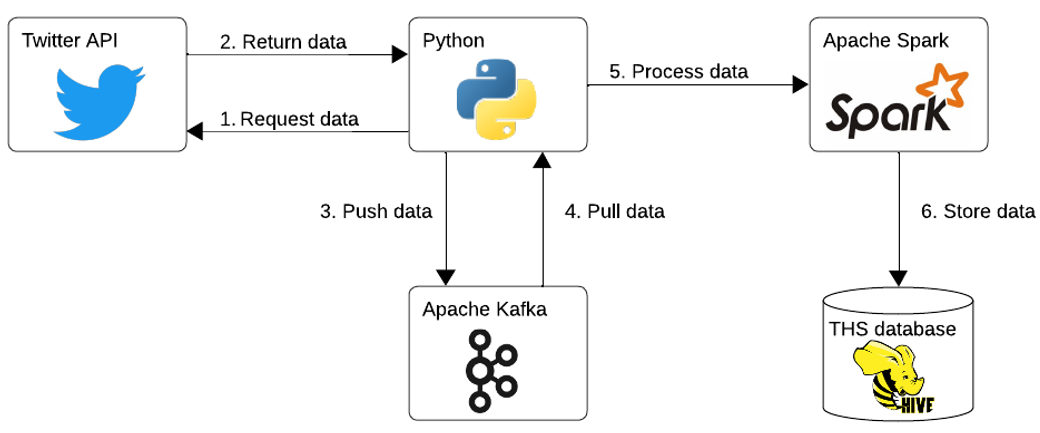
\includegraphics[width=1\linewidth]{images/ths_architecture.png}
        \caption{THS Architecture}
        \label{ths_architecture}
\end{figure}

 
Later the project was updated to find similarities between tweets \cite{9581175}. This new version tested convolutional neural networks (CNN) and recurrent neural networks to classify how closely related are two different tweets.
They used a ranking method that gave a higher score if two randomly selected tweets were similar. The agent received an input of triplets where the first element was compared against the other two elements.
The system trained on two data types: raw tweets and cleaned tweets. This latter had stop-words removed and a lemmatization process. Cleaned tweets proved a higher accuracy in the recurrent neural network
for regular LSTM and bidirectional networks; in contrast, the raw tweet had a better result in CNN validation. All three models had similar results; the highest validation accuracy was the regular LSTM with 90\%,
followed by the other two with 87\%. Nonetheless, the training time for the CNN was the fastest, with regular LSTM in second place and the slowest being the bidirectional LSTM network. 


  \begin{figure}[!h]
    \centering
        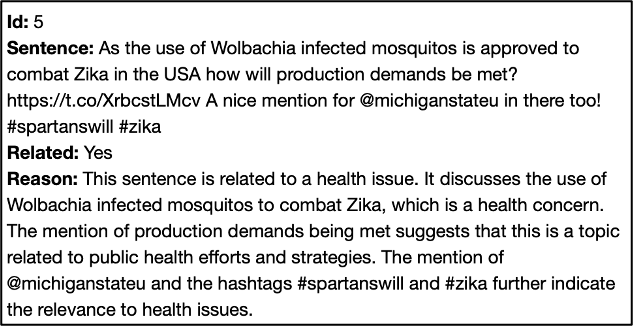
\includegraphics[width=0.8\linewidth]{images/base_gpt_health.png}
        \caption{ChatGPT Classification Example – Health Related}
        \label{gpt_health}
\end{figure}

However, both of these experiments removed special characters or elements from the original text. By then, tweets had a limitation of characters, making each one of the crucial the context. Removing special
characters, could remove information that the author of the text intended. We can have the example in Figure \ref{gpt_health}, where a based model GPT classified a text. The model uses the hashtag and mention
as context to determine if the text is health related or not. This is a good presumption, but these platforms' users could use hashtags or mentions that are not relevant to the text. 



